% Part 3 of Day 1: The edge AI workflow.
%
% Topics of the syllabus: data, training, optimization, conversion,
% deployment, monitoring; hybrid architectures; course map; live
% demonstration of keyword spotting on the XIAOML Kit. Exercise: predict
% which of three models fits in 256 KB of RAM.
%
% Preparation for the instructor: the live demonstration needs one XIAOML Kit
% with a keyword spotting sketch (classes YES, NO, NOISE, UNKNOWN) that shows
% the result on the display. The kit chapter "Keyword Spotting (KWS)" of
% "Machine Learning Systems" gives the steps. Build the sketch with the
% option "OPI PSRAM".

\theorypart{The edge AI workflow}%
  {predict which of three models fits in 256 KB of RAM}

% ------------------------------------------------------------------ workflow
\begin{frame}{The edge AI workflow}
  \begingroup\centering
  \begin{tikzpicture}[font=\small, >={Stealth[length=5pt]},
      st/.style={draw=darkcyan, line width=0.8pt, rounded corners=3pt,
                 fill=boxgray, minimum width=2.7cm, minimum height=1.15cm,
                 align=center},
      sub/.style={font=\footnotesize, text=coolgray}]
    \node[st] (d) at (0,0)      {\textbf{1. Data}\\[-1pt]{\footnotesize collect and label}};
    \node[st] (t) at (3.6,0)    {\textbf{2. Training}\\[-1pt]{\footnotesize fit the model}};
    \node[st] (o) at (7.2,0)    {\textbf{3. Optimization}\\[-1pt]{\footnotesize make it small}};
    \node[st] (c) at (7.2,-2.3) {\textbf{4. Conversion}\\[-1pt]{\footnotesize format of the runtime}};
    \node[st] (p) at (3.6,-2.3) {\textbf{5. Deployment}\\[-1pt]{\footnotesize run on the device}};
    \node[st] (m) at (0,-2.3)   {\textbf{6. Monitoring}\\[-1pt]{\footnotesize watch the device}};
    \draw[->] (d) -- (t);
    \draw[->] (t) -- (o);
    \draw[->] (o) -- (c);
    \draw[->] (c) -- (p);
    \draw[->] (p) -- (m);
    \draw[->, cardinalred, dashed, line width=0.8pt] (m) --
      node[right, font=\footnotesize, align=left] {new data,\\new model} (d);
  \end{tikzpicture}\par\endgroup
  \vskip 0.6em
  \begin{itemize}
    \item A cloud project trains a model and serves it. An edge project adds
          two stages: optimization and conversion.
    \item The workflow is a loop. Deployment is the start of the feedback,
          not the end of the project.
  \end{itemize}
\end{frame}

\begin{frame}{Each stage has a place and an output}
  \small
  \renewcommand{\arraystretch}{1.35}
  \begin{tabular}{@{}L{0.20\textwidth}L{0.27\textwidth}L{0.44\textwidth}@{}}
    \toprule
    \textbf{Stage} & \textbf{Where it runs} & \textbf{Output} \\
    \midrule
    1. Data         & Sensor of the device & A labelled data set \\
    2. Training     & Laptop or cloud      & A \code{float32} model with a
                                             known accuracy \\
    3. Optimization & Laptop or cloud      & A smaller model. You measure
                                             its accuracy again. \\
    4. Conversion   & Laptop               & A model file for the runtime of
                                             the device \\
    5. Deployment   & Device               & An application: sensor input,
                                             model, action \\
    6. Monitoring   & Device and network   & Measured values, logs, new
                                             data \\
    \bottomrule
  \end{tabular}
  \vskip 0.8em
  \keypoint{Training runs where the computation is. Inference runs where the
    data is. This pattern is the train-serve split.}
\end{frame}

\begin{frame}{The device constraints come first}
  \begingroup\centering
  \begin{tikzpicture}[font=\footnotesize, x=1cm, y=0.068cm]
    % y unit: 1 = cost factor 1
    \draw[coolgray] (-0.2,0) -- (9.6,0);
    \fill[treegreen!60]   (0.1,0) rectangle (1.1,1);
    \fill[treegreen!60]   (1.7,0) rectangle (2.7,2);
    \fill[darkcyan!55]    (3.3,0) rectangle (4.3,4);
    \fill[darkcyan!55]    (4.9,0) rectangle (5.9,8);
    \fill[cardinalred!60] (6.5,0) rectangle (7.5,16);
    \fill[cardinalred!60] (8.1,0) rectangle (9.1,32);
    \node[above] at (0.6,1)  {1$\times$};
    \node[above] at (2.2,2)  {2$\times$};
    \node[above] at (3.8,4)  {4$\times$};
    \node[above] at (5.4,8)  {8$\times$};
    \node[above] at (7.0,16) {16$\times$};
    \node[above] at (8.6,32) {32$\times$};
    \node[below, align=center] at (0.6,0) {problem\\definition};
    \node[below, align=center] at (2.2,0) {data\\collection};
    \node[below, align=center] at (3.8,0) {model\\development};
    \node[below, align=center] at (5.4,0) {evaluation};
    \node[below, align=center] at (7.0,0) {deployment};
    \node[below, align=center] at (8.6,0) {monitoring};
    \node[anchor=west, align=left] at (0,27) {Cost to correct a decision,\\
      by the stage where you find the error};
  \end{tikzpicture}\par\endgroup
  \vskip 0.3em
  \begin{itemize}
    \item The book gives a rule: the cost of a correction doubles with each
          stage.
    \item Example: after training, you find that the model needs 300 KB of
          RAM. The device has 256 KB. You start the model design again.
  \end{itemize}
  \keypoint{Write the budgets of the device before you collect data: flash,
    RAM, latency, energy.}
  \source{\emph{Machine Learning Systems}, Volume I, chapter 3.}
\end{frame}

% ------------------------------------------------------------------ stages
\begin{frame}{Stage 1: data}
  \begin{columns}[T]
    \begin{column}{0.52\textwidth}
      \begin{itemize}
        \item The data set is the critical part of the workflow.
        \item Record the data with the same type of sensor that the device
              uses.
        \item Record in the conditions of the application: position,
              noise, light, different persons.
        \item Add classes for ``nothing'' and for ``unknown''. The device
              sees these inputs most of the time.
      \end{itemize}
    \end{column}
    \begin{column}{0.44\textwidth}
      \begin{block}{Questions of the device}
        \begin{itemize}
          \item Which sampling rate can the sensor give?
          \item How long is one input window?
          \item How large is one input in RAM?
        \end{itemize}
      \end{block}
      \begin{block}{In this course}
        Day 2: you record motion data with the IMU of the XIAOML Kit.
      \end{block}
    \end{column}
  \end{columns}
\end{frame}

\begin{frame}{Stage 2: training}
  \begin{columns}[T]
    \begin{column}{0.52\textwidth}
      \begin{itemize}
        \item Training runs on a laptop or in the cloud. It needs the
              backward pass and many passes through the data.
        \item The device does only the forward pass.
        \item Select a model that can meet the three budgets of the device
              (Part~2). A model that is too large stays too large.
        \item Keep the pre-processing identical in training and on the
              device.
      \end{itemize}
    \end{column}
    \begin{column}{0.44\textwidth}
      \begin{block}{Output of this stage}
        \begin{itemize}
          \item A \code{float32} model
          \item The accuracy on test data
          \item Parameters, operations, and peak activation memory
        \end{itemize}
      \end{block}
      \begin{block}{In this course}
        Days 3, 5, and 8: you train small models with Keras, Edge Impulse
        Studio, and Ultralytics.
      \end{block}
    \end{column}
  \end{columns}
\end{frame}

\begin{frame}{Stage 3: optimization}
  \renewcommand{\arraystretch}{1.2}
  \begin{tabular}{@{}L{0.24\textwidth}L{0.42\textwidth}L{0.22\textwidth}@{}}
    \toprule
    \textbf{Method} & \textbf{What it changes} & \textbf{In this course} \\
    \midrule
    Quantization & The data type: \code{float32} to \code{int8}. Four times
                   less flash and RAM. & Day 4 \\
    Pruning      & It removes weights or channels. & Day 6 \\
    Knowledge distillation & A small model learns from a large model.
                 & Day 6 \\
    Efficient design & Blocks with a lower cost (Part~2). & Days 1 and 6 \\
    \bottomrule
  \end{tabular}
  \vskip 0.8em
  \begin{itemize}
    \item Each method exchanges accuracy for size, latency, or energy.
    \item Measure the accuracy and the three budgets before and after each
          step.
  \end{itemize}
\end{frame}

\begin{frame}{Stage 4: conversion}
  \begingroup\centering
  \begin{tikzpicture}[font=\footnotesize, >={Stealth[length=5pt]},
      b/.style={draw=coolgray, rounded corners=3pt, fill=boxgray,
                minimum width=2.05cm, minimum height=0.9cm, align=center},
      r/.style={b, draw=cardinalred, line width=0.8pt}]
    \node[anchor=west, text=coolgray] at (-1.05,0.85)
      {\textbf{Microcontroller (XIAOML Kit)}};
    \node[b] (k) at (0,0)   {Keras model};
    \node[b] (l) at (2.8,0) {LiteRT file\\\code{.tflite}};
    \node[b] (h) at (5.6,0) {C array in a\\header file};
    \node[r] (m) at (8.4,0) {TensorFlow\\Lite Micro};
    \draw[->] (k) -- (l);
    \draw[->] (l) -- (h);
    \draw[->] (h) -- (m);
    \node[anchor=west, text=coolgray] at (-1.05,-1.25)
      {\textbf{Linux device (Raspberry Pi 5)}};
    \node[b] (p) at (0,-2.1)   {PyTorch model};
    \node[b] (o) at (2.8,-2.1) {ONNX file\\\code{.onnx}};
    \node[r] (q) at (8.4,-2.1) {ONNX Runtime,\\LiteRT, NCNN};
    \draw[->] (p) -- (o);
    \draw[->] (o) -- (q);
  \end{tikzpicture}\par\endgroup
  \vskip 0.5em
  \begin{itemize}
    \item The training framework does not run on a small device. A runtime
          reads the converted model and executes it.
    \item A microcontroller has no file system for the model. The model is
          a constant array in the firmware.
    \item Risk: the runtime does not support an operator of the model.
          Check this before you train for a long time.
  \end{itemize}
\end{frame}

\begin{frame}{Stage 5: deployment}
  \begingroup\centering
  \begin{tikzpicture}[font=\footnotesize, >={Stealth[length=5pt]},
      b/.style={draw=coolgray, rounded corners=3pt, fill=boxgray,
                minimum width=1.75cm, minimum height=0.9cm, align=center},
      r/.style={b, draw=cardinalred, line width=0.8pt},
      e/.style={font=\scriptsize, text=coolgray, align=center,
                text width=1.9cm}]
    \node[b] (s) at (0,0)   {Sensor};
    \node[b] (f) at (2.15,0) {Pre-\\processing};
    \node[r] (m) at (4.3,0) {Model and\\runtime};
    \node[b] (q) at (6.45,0) {Post-\\processing};
    \node[b] (a) at (8.6,0) {Action};
    \draw[->] (s) -- (f);
    \draw[->] (f) -- (m);
    \draw[->] (m) -- (q);
    \draw[->] (q) -- (a);
    \node[e] at (0,-0.95)    {microphone, 16 kHz};
    \node[e] at (2.15,-0.95) {audio features};
    \node[e] at (4.3,-0.95)  {small CNN, \code{int8}};
    \node[e] at (6.45,-0.95) {probability above a threshold?};
    \node[e] at (8.6,-0.95)  {LED, display, message};
  \end{tikzpicture}\par\endgroup
  \vskip 0.4em
  \begin{itemize}
    \item The device runs a pipeline, not only a model. Each step needs
          time and memory.
    \item Microcontroller: one firmware image holds the program, the
          runtime, and the model.
    \item Linux device: a program loads the runtime and the model file.
    \item Then you measure on the device: latency, memory, and energy
          (Day 9).
  \end{itemize}
\end{frame}

\begin{frame}{Stage 6: monitoring}
  \begin{columns}[c]
    \begin{column}{0.46\textwidth}
      \centering
      \begin{tikzpicture}[font=\footnotesize, x=0.36cm, y=0.05cm,
          >={Stealth[length=5pt]}]
        % x: months 0 to 12. y: accuracy in percent, 60 to 100, shifted.
        \draw[->, coolgray] (0,0) -- (13,0) node[below left] {months};
        \draw[->, coolgray] (0,0) -- (0,58) node[above right] {accuracy};
        \draw[darkcyan, line width=1pt] (0,48) -- (12,48);
        \draw[cardinalred, line width=1pt]
          (0,48) .. controls (4,47) and (7,40) .. (12,24);
        \node[darkcyan, anchor=south west] at (4.2,48) {classic software};
        \node[cardinalred, anchor=west, align=left] at (5.2,20)
          {deployed\\model};
      \end{tikzpicture}
    \end{column}
    \begin{column}{0.52\textwidth}
      \begin{itemize}
        \item Classic software fails with an error message.
        \item A model fails with no message. The world changes, and the
              accuracy decreases.
        \item The book gives a loss of 10 to 15\,\% in some months, with no
              change of the code.
        \item An edge device has no operator who watches it. It must report
              its condition.
      \end{itemize}
    \end{column}
  \end{columns}
  \vskip 0.5em
  \keypoint{Send measured values from the device: confidence, latency,
    temperature. Days 12 and 13 show the method.}
  \source{\emph{Machine Learning Systems}, Volume I, chapter 1. The curve is
    a sketch, not measured data.}
\end{frame}

% ------------------------------------------------------------------- hybrid
\begin{frame}{Hybrid architectures: one product, three paradigms}
  \begingroup\centering
  \begin{tikzpicture}[font=\footnotesize, >={Stealth[length=5pt]},
      t/.style={draw, line width=0.8pt, rounded corners=3pt, fill=boxgray,
                minimum width=2.6cm, minimum height=1.9cm, align=center}]
    \node[t, draw=cardinalred] (a) at (0,0)
      {\textbf{Wake word}\\TinyML\\less than 1 mW\\10 ms};
    \node[t, draw=coolgray] (b) at (3.7,0)
      {\textbf{Speech to text}\\Mobile\\3 to 5 W\\80 ms};
    \node[t, draw=darkcyan] (c) at (7.4,0)
      {\textbf{Language model}\\Cloud\\700 W\\110 ms};
    \draw[->] (a) -- node[above, font=\scriptsize] {trigger} (b);
    \draw[->] (b) -- node[above, font=\scriptsize] {text} (c);
  \end{tikzpicture}\par\endgroup
  \vskip 0.5em
  \begin{itemize}
    \item A voice assistant is three systems. Each stage runs where its
          constraint costs the least.
    \item The wake word model is always on. Thus it must use very little
          power.
    \item The language model is too large for the device. Thus it runs in
          the cloud.
    \item The total budget is 200 ms. The network is the part that varies
          most.
  \end{itemize}
  \source{\emph{Machine Learning Systems}, Volume I, chapters 1 and 2.}
\end{frame}

\begin{frame}{Three patterns for a hybrid system}
  \small
  \renewcommand{\arraystretch}{1.35}
  \begin{tabular}{@{}L{0.21\textwidth}L{0.34\textwidth}L{0.35\textwidth}@{}}
    \toprule
    \textbf{Pattern} & \textbf{What it does} & \textbf{Select it when} \\
    \midrule
    Train-serve split & Training in the cloud, inference on the device.
      & Training needs a scale that inference does not need. \\
    Hierarchical processing & Each tier filters the data and sends less to
      the next tier. & The data volume is larger than the capacity of the
      connection. \\
    Progressive deployment & One model family, compressed for each tier.
      & The same function is necessary on devices of different size. \\
    \bottomrule
  \end{tabular}
  \vskip 0.6em
  \normalsize
  A special case of hierarchical processing: a small model on the device
  answers when its confidence is high. It sends only the difficult inputs
  to a larger model.
\end{frame}

\begin{frame}{The hybrid system of this course}
  \begingroup\centering
  \begin{tikzpicture}[font=\footnotesize, >={Stealth[length=5pt]},
      n/.style={draw, line width=0.8pt, rounded corners=3pt, fill=boxgray,
                minimum height=1.9cm, align=flush center},
      l/.style={font=\scriptsize, align=center}]
    \node[n, draw=cardinalred, text width=2.5cm] (x) at (0,0)
      {\textbf{XIAOML Kit}\\TinyML\\sensor, small model\\local decision};
    \node[n, draw=treegreen, text width=2.5cm] (p) at (4.5,0)
      {\textbf{Raspberry Pi 5}\\Edge ML\\larger models\\broker, dashboard};
    \node[n, draw=coolgray, dashed, text width=1.9cm] (c) at (7.9,0)
      {\textbf{Cloud}\\not necessary for operation};
    \draw[->] ([yshift=4pt]x.east) -- node[l, above] {MQTT:\\results}
      ([yshift=4pt]p.west);
    \draw[->] ([yshift=-4pt]p.west) -- node[l, below] {commands}
      ([yshift=-4pt]x.east);
    \draw[->, dashed] (p) -- (c);
  \end{tikzpicture}\par\endgroup
  \vskip 0.5em
  \begin{itemize}
    \item Week 1: a model on the microcontroller makes a decision at the
          sensor.
    \item Week 2: the Raspberry Pi runs models that are too large for the
          microcontroller.
    \item Week 3: the two boards exchange messages. The system continues to
          work with no internet connection.
    \item You train on a laptop and deploy on the boards. This is the
          train-serve split.
  \end{itemize}
\end{frame}

\begin{frame}{Course map}
  \begingroup\centering
  \begin{tikzpicture}[font=\scriptsize,
      d/.style={draw=coolgray, rounded corners=2pt, fill=boxgray,
                minimum width=2.0cm, minimum height=1.05cm,
                align=flush center, text width=1.85cm, inner sep=1pt},
      w/.style={anchor=west, font=\footnotesize\bfseries, text=coolgray}]
    \node[w] at (-1.05,0.8) {Week 1: XIAOML Kit};
    \node[d, draw=cardinalred, line width=0.8pt] at (0,0)
      {\textbf{Day 1}\\Landscape\\and budgets};
    \node[d] at (2.1,0) {\textbf{Day 2}\\Data};
    \node[d] at (4.2,0) {\textbf{Day 3}\\Train, convert,\\deploy};
    \node[d] at (6.3,0) {\textbf{Day 4}\\Optimize:\\quantization};
    \node[d] at (8.4,0) {\textbf{Day 5}\\Deploy:\\audio, vision};
    \node[w] at (-1.05,-1.05) {Week 2: laptop and Raspberry Pi 5};
    \node[d] at (0,-1.85)   {\textbf{Day 6}\\Optimize: prune,\\distil};
    \node[d] at (2.1,-1.85) {\textbf{Day 7}\\Convert:\\runtimes};
    \node[d] at (4.2,-1.85) {\textbf{Day 8}\\Train, deploy:\\detection};
    \node[d] at (6.3,-1.85) {\textbf{Day 9}\\Measure:\\benchmarks};
    \node[d] at (8.4,-1.85) {\textbf{Day 10}\\Deploy:\\language models};
    \node[w] at (-1.05,-2.9) {Week 3: both boards};
    \node[d] at (0,-3.7)   {\textbf{Day 11}\\Connect:\\RTSP};
    \node[d] at (2.1,-3.7) {\textbf{Day 12}\\Connect:\\MQTT};
    \node[d] at (4.2,-3.7) {\textbf{Day 13}\\Monitor};
    \node[d] at (6.3,-3.7) {\textbf{Day 14}\\Design for\\production};
    \node[d] at (8.4,-3.7) {\textbf{Day 15}\\Capstone};
  \end{tikzpicture}\par\endgroup
  \vskip 0.5em
  \keypoint{Each day adds one stage of the workflow, or it measures a stage.
    The capstone project uses all six stages.}
\end{frame}

% --------------------------------------------------------------- live demo
\begin{frame}{Live demonstration: keyword spotting}
  \begingroup\centering
  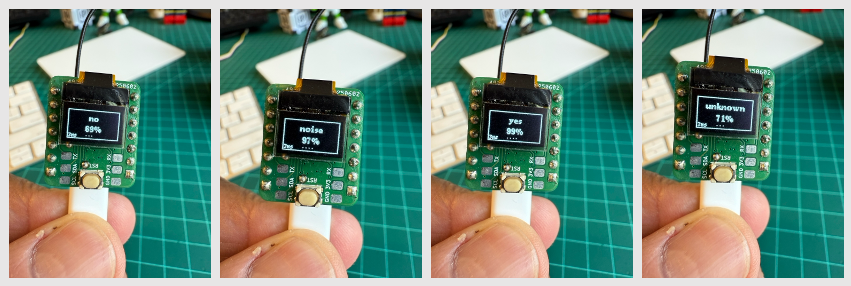
\includegraphics[width=0.92\textwidth]{images/day01/kws-on-the-kit.png}\par
  \endgroup
  \vskip 0.3em
  \begin{columns}[T]
    \begin{column}{0.47\textwidth}
      \small
      The kit listens continuously. It classifies one second of sound:
      YES, NO, NOISE, or UNKNOWN. The display shows the class and the
      confidence.
    \end{column}
    \begin{column}{0.47\textwidth}
      \begin{block}{Predict before the demonstration}
        \small
        \begin{enumerate}
          \item Does it work with Wi-Fi off?
          \item How much time passes from the word to the result?
          \item What does it show for a different word?
        \end{enumerate}
      \end{block}
    \end{column}
  \end{columns}
  \source{Photograph: kit chapter ``Keyword Spotting'' of \emph{Machine
    Learning Systems} (CC BY-NC-SA 4.0).}
\end{frame}

\begin{frame}{The demonstration through the six stages}
  \small
  \renewcommand{\arraystretch}{1.35}
  \begin{tabular}{@{}L{0.22\textwidth}L{0.70\textwidth}@{}}
    \toprule
    \textbf{Stage} & \textbf{Keyword spotting on the kit} \\
    \midrule
    1. Data         & Speech Commands data set and own recordings. Audio
                      with 16 kHz and 16 bits. Four classes. \\
    2. Training     & Edge Impulse Studio. Audio features (MFCC) and a
                      small CNN with two convolution blocks. \\
    3. Optimization & Quantization to \code{int8}. \\
    4. Conversion   & The Studio makes an Arduino library with the model
                      and TensorFlow Lite Micro. \\
    5. Deployment   & One sketch: microphone, features, model, threshold,
                      display. The build needs PSRAM. \\
    6. Monitoring   & The display shows the class and the confidence. No
                      data leaves the kit. \\
    \bottomrule
  \end{tabular}
  \vskip 0.6em
  \normalsize
  The source reports an accuracy of about 87\,\% on its test data. You build
  this system on Day 5.
  \source{Kit chapter ``Keyword Spotting'' of \emph{Machine Learning
    Systems}.}
\end{frame}

% ----------------------------------------------------------------- fit check
\begin{frame}{Before you deploy: does the model fit?}
  \begin{columns}[T]
    \begin{column}{0.47\textwidth}
      \begin{block}{Flash}
        model size $+$ program $\leq$ flash
        \vskip 0.3em
        model size $=$ parameters $\times$ bytes for each parameter
      \end{block}
    \end{column}
    \begin{column}{0.47\textwidth}
      \begin{block}{RAM}
        peak activation memory $+$ program data $\leq$ RAM
        \vskip 0.3em
        peak $=$ values $\times$ bytes for each value
      \end{block}
    \end{column}
  \end{columns}
  \vskip 0.6em
  \begin{itemize}
    \item The program also needs RAM: the stack, the sensor buffer, the
          runtime.
    \item Do not use the complete RAM for the tensors. In the lab you
          measure the RAM that a sketch with no model uses.
    \item Check the two budgets. One number is not sufficient.
  \end{itemize}
  \vskip 0.3em
  \keypoint{Device of the exercise: a Cortex-M4 microcontroller with 1 MB of
    flash and 256 KB of RAM.}
\end{frame}

% -------------------------------------------------------------------- exercise
\exerciseframe{which model fits in 256 KB of RAM?}{%
  The device has 256 KB of RAM and 1 MB of flash.
  \vskip 0.4em
  {\small
  \renewcommand{\arraystretch}{1.25}
  \begin{tabular}{@{}L{0.37\textwidth}lrr@{}}
    \toprule
    \textbf{Model} & \textbf{Type} & \textbf{Parameters}
      & \textbf{Peak (values)} \\
    \midrule
    A. Fully connected, 784-128-64-10 & \code{float32} & 109\,386 & 912 \\
    B. Example CNN of Part 2 & \code{float32} & 24\,234 & 64\,512 \\
    C. MobileNetV2, image $224 \times 224$ & \code{int8} & 3.5 million
      & 1.5 million \\
    \bottomrule
  \end{tabular}\par}
  \vskip 0.5em
  \begin{enumerate}
    \item Predict first, with no calculation: which models fit in the RAM?
    \item Calculate the peak activation memory and the model size of each
          model in KB.
    \item Which model has the most parameters of the models that fit?
  \end{enumerate}
  Work with your neighbour for 7 minutes.
}

\answerframe{which model fits in 256 KB of RAM?}{%
  {\small
  \renewcommand{\arraystretch}{1.25}
  \begin{tabular}{@{}lrrl@{}}
    \toprule
    \textbf{Model} & \textbf{Peak in RAM} & \textbf{Model size}
      & \textbf{Result} \\
    \midrule
    A & 3.6 KB  & 427 KB & fits \\
    B & 252 KB  & 95 KB  & RAM too small \\
    C & 1470 KB & 3.3 MB & RAM and flash too small \\
    \bottomrule
  \end{tabular}\par}
  \vskip 0.5em
  \begin{itemize}
    \item A has 4.5 times more parameters than B, but only A fits. The
          parameters do not show the RAM.
    \item B needs 252 KB for the tensors. No RAM remains for the program.
          In \code{int8}, B needs 63 KB and it fits.
    \item C fails in the first layers. Its largest tensors have 1.5 million
          values. Quantization is not sufficient: the model needs a smaller
          image or a different design.
  \end{itemize}
}
